\section{Augmentation of Stellar Grid}\label{sec:augmentation}
In this section, we demonstrate our training process for a 3-demission and a 5-demission grid.  

\subsection{GPR models with 3D inputs}

\subsection{GPR models with 5D inputs}

\begin{figure*}
	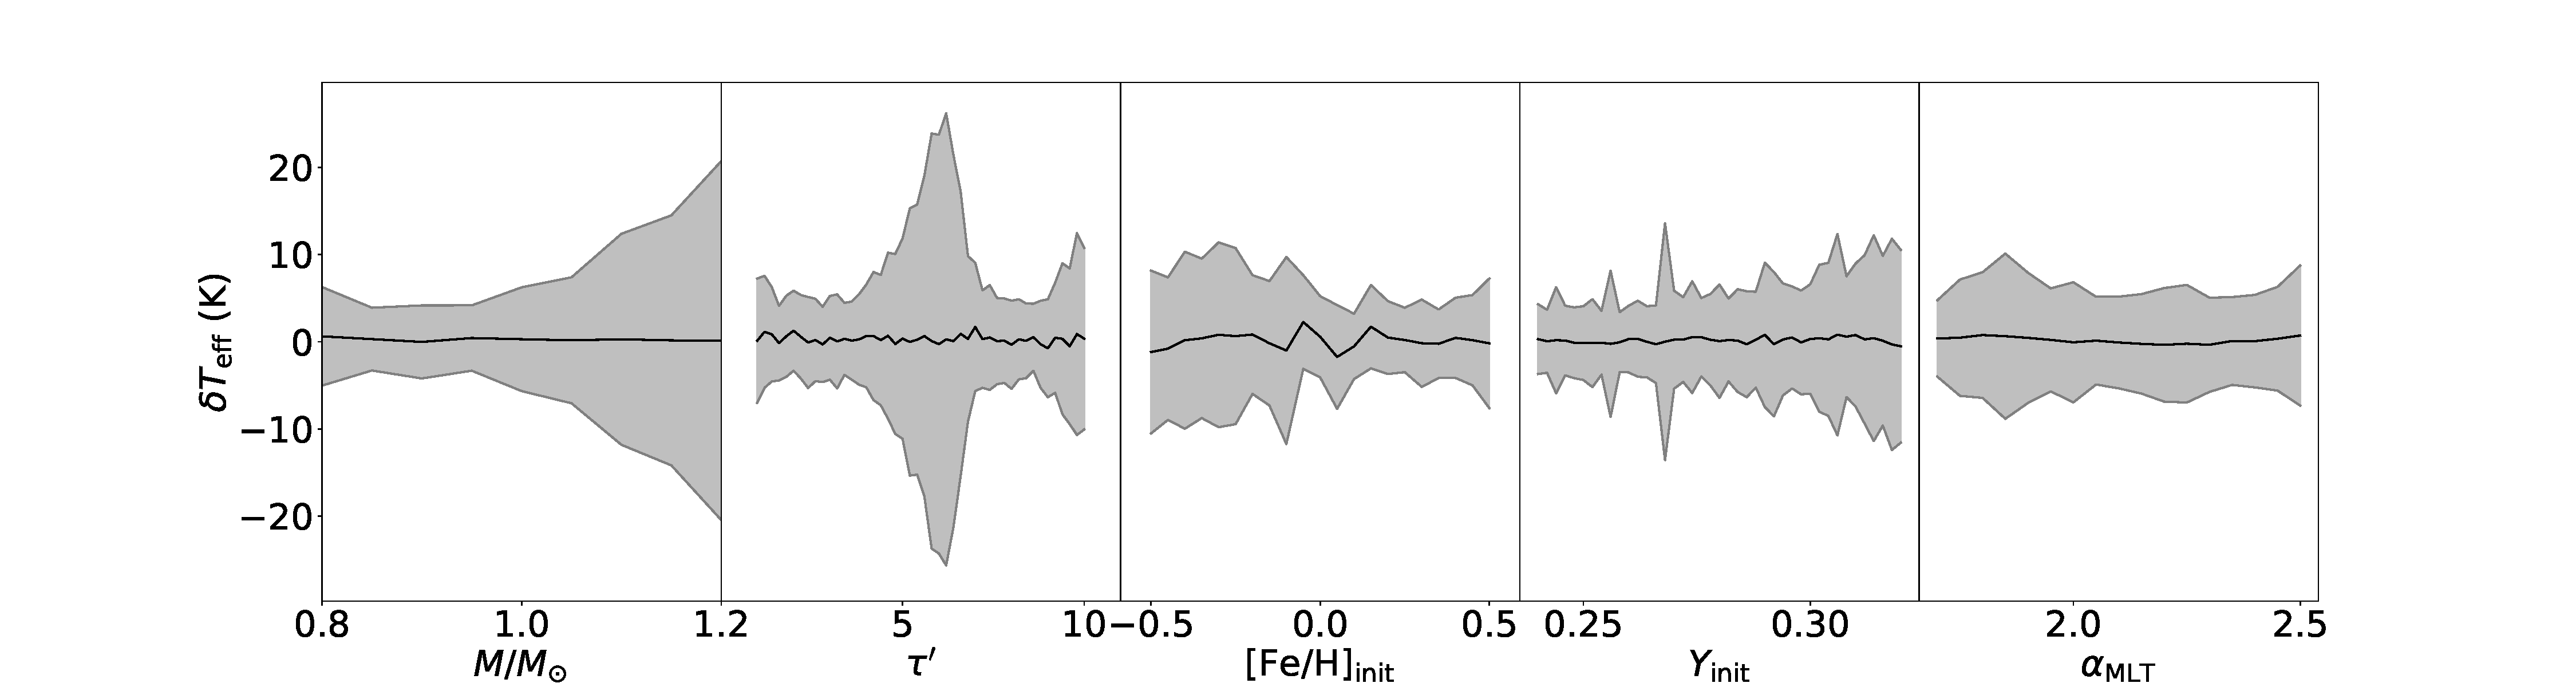
\includegraphics[width=1.1\textwidth]{validataion_vs_inputs_teff.pdf}
    \caption{}
    \label{fig:5dresults}
\end{figure*}


\begin{table*}
	\centering
	\caption{Training and validating for the 5D model grid}
	\label{tab:gpdetails}
	\begin{tabular}{lcll} % four columns, alignment for each
		\hline
		 GPR model input &\multicolumn{1}{l}{GPR model output} & \multicolumn{1}{c}{GPR model combination and kernels}& 
		  \multicolumn{1}{c}{Validation errors (\%)}\\ 
		 \hline
		 $M$, $t_{\rm frac}$, [Fe/H]$_{\rm init}$, $Y_{\rm init}$, $\alpha_{\rm MLT}$ & $T_{\rm eff}$ (K) &M0(MLP)+M1(MLP)& 0.05/0.3/1\\
		 &$\log g$ (dex)  & M0(MLP)+M1(Mat32)+M2(EXP) &0.01/0.07/0.3\\
		 &$R$ ($R_{\odot}$) & M0(MLP)+M1(Mat32)+M2(EXP) &0.07/0.4/2\\
		  &$\Delta\nu$ ($\mu$Hz) & M0(MLP)+M1(Mat32)+M2(EXP) &0.1/0.7/3\\
		  &($Z/X$)$_{\rm surf}$ & M0(MLP)+M1(Mat32)+M2(RBF) & 0.1/1/6\\
		  &$\tau$ (Gyr) & M0(MLP)+M1(Mat32)+M2(RBF) & 0.1/1/14\\
       \hline
	\end{tabular}
\end{table*}


\section{Systematical Uncertainties of GPR Models}\label{sec:sys}

\section{Modeling stars with GPR models}

%\subsubsection{Three Fake Stars}

%\subsubsection{The Sun}

%\subsubsection{Six {\em Kepler} Dwarfs and Subgiants}

\begin{itemize}
\item Accuracy goes down. Because the multiple-demission space size increase while the training dataset has a limitation of 10,000 points.  
\item We hence need to divide the grid into small chunks and train each chunk separately.  (illustrate how chunks are divided)
\item  show training and validation results in a fancy way. 
\end{itemize}









